%!TEX root = ../main.tex

\chapter{学位论文排版元素}

通过阅读上一章节,
相信您已基本配置好了自己的编辑环境,
了解了如何正确编写各级章节、段落和子段落,
容易引起编译出错的逃逸字符。

从上一章出现过的有序列表、外部图片和代码环境中,
您应该已经发现,
使用命令\texttt{$\backslash$begin\{xxxx\}}可以开始一段新的布局环境。
这一章将系统地阐述计算机类的学位论文需要排版的元素的编写方法。
主要包括以下排版要素:
\begin{itemize}
    \item 列表环境(包括有序、无序、定义三种列表)
    \item 插图和表格
    \item 代码环境
    \item 数学和算法环境
\end{itemize}

这一章只涉及为完成此排版环境的宏包的最基本使用方法,
本章尽量覆盖论文写作中的大部分场景,
如有特殊需求,请仔细阅读相关宏包手册并求助于国内外TeX社区及问答网站。

\section{列表环境}

列表环境有三种,
类似与HTML的\texttt{<ol>},
\texttt{<ul>},\texttt{<dl>}
三个标签。
以下是一个定义列表环境:
\begin{description}
    \item[有序列表] enumerate 默认从阿拉伯数字1开始编号,如需更改请搜“重定义列表”
    \item[无序列表] itemize 默认圆点标记,尽量少用此类列表
    \item[定义列表] description 语义上用于作一系列简短的解释
\end{description}

列表可以嵌套,比如:
\begin{enumerate}
	\item 第一级列表
	\item 第一级列表
	\begin{enumerate}
		\item 第二级列表
		\item 第二级列表
        \begin{itemize}
            \item 第三级列表
            \item 第三级列表
		\end{itemize}
		\item 第二级列表
		\item 第二级列表
	\end{enumerate}
\end{enumerate}

\section{插图环境和浮动体}

相信您在上一章的探索学习中已经基本掌握了如何插入图片的方法,
但可能仍存疑虑。
所以现在先简单介绍浮动体的概念以助您理解插图环境的布局规则,
最后再介绍子图的排布以应对您更高的布局需求。
% 关于绘图,本文将在后续章节讲述
% 活用引用,让评阅老师随处移动
关于图的绘制,本文将在\ref{how-to-plot} 继续讲述。

当一个图片或表格太大在当前页面无法继续排布时,
一种解决方案就是新开一页再排布(Word 默认使用此种)。
这个方法在页面上留下分空白,十分不美观。
\LaTeX 的默认解决方案是把它们“浮动”到下一页,
与此同时使用后续正文文本填充当前的空白。

插图和表格在\LaTeX 排版中被默认当成浮动体对待,
当排版引擎试图放置一个浮动体时,它将遵循以下规则:
\begin{enumerate}
    \item 浮动体的布局大小不得超过版心的大小,否则抛出Overfull Page错误
    \item 浮动体只会向后浮动,不会向前浮动
    \item 浮动体默认按照 h $\to$ t $\to$ b $\to$ p 的规则布局
    \begin{description}
        \item[h] 当前位置,如果本页所剩空间不够,这一参数无效
        \item[t] 浮动到下一页顶部
        \item[b] 浮动到下一页底部(脚注之下)
        \item[p] 浮动到一个允许出现浮动体的页面上
        \item[!] 忽略浮动体放置的大多数内部参数\footnote{作者也不太懂}
    \end{description}
    \item 设置 htbp 参数的顺序不会影响默认的规则顺序
\end{enumerate}

在实践中,一般选用浮动规则[htbp], [tbp], [htp], [tp] 来完成浮动体布局。
请不要使用单一参数布局,这样极有可能出现难解的浮动问题。
不适当的浮动规则参数将导致浮动对象被放进一个队列中等待布局,
这个队列的默认大小是18,如果队列超限,编译中会抛出一个Too Many Unprocessed Floats错误。
如果一页图片太多,甚至几乎占满一个版心,
您可以通过\texttt{$\backslash$clearpage}命令强制在此处必须排版完所有浮动体
再排版之后内容,关于清除浮动等复杂主题,这里不再展开。
此处只能建议插图尺寸不宜过大,插图密度不宜过大。
考虑到图文混排的最佳视觉要求,
可以待论文内容稳定下之后,仔细调整插图代码的位置,
通过前置插图代码,强行“向后浮动”,保证插图和引用处足够近。

关于模板对浮动体的设置,参看\texttt{zjuthesis.cls},
搜索关键字“浮动体”找到对应配置。
图片引用路径在\texttt{zjuthesis.cls}里定义的\texttt{graphicspath}里,
默认情况下\\\texttt{$\backslash$includegraphics}命令从论文源码根目录搜索引用的图片,
如果先在根目录里匹配到文件名,则不再前往定义路径搜索,
当引擎无法找到您指定的图片资源时,会导致编译错误。
注意引用的文件名包括文件后缀。

% 现在你可以随意更动此插图代码的位置来感受一下浮动体布局的规则
\begin{figure}[htbp]
	\centering
	\begin{subfigure}[b]{.45\textwidth}  % 注意此处的尺寸控制
		\centering
		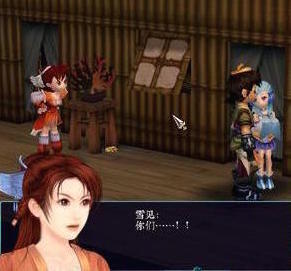
\includegraphics[width = \textwidth]{xuejian.jpg}
		\caption{仙三}\label{fig:subfig-samp1}
	\end{subfigure}
	\begin{subfigure}[b]{.45\textwidth}
		\centering
		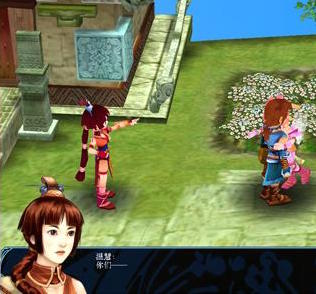
\includegraphics[width = \textwidth]{wenhui.jpg}
		\caption{仙三外}\label{fig:subfig-samp2}
	\end{subfigure}
	\begin{subfigure}[b]{.45\textwidth}
		\centering
		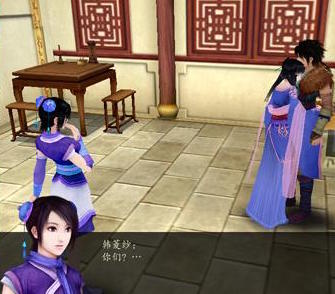
\includegraphics[width = \textwidth]{lingsha.jpg}
		\caption{仙四}\label{fig:subfig-samp3}
	\end{subfigure}
	\caption{仙剑白学传}\label{fig:subfig-samp}
\end{figure}

接下来描述一下子图的编写,
在实际论文撰写过程中,
经常遇到需要比较几组实验数据或场景的需求。
此时,合乎语义的做法是为不同的组设置子图,
而不是分别设图。

多个子图组成一个单独的浮动体进行布局,
共用一个总图题总引用,并可以有各自单独的子图题和交叉引用。
本模板使用subcaption 宏包处理子图排版问题,如\autoref{fig:subfig-samp} 所示
\footnote{不要在正式论文排版过程中使用彩色区分类别,论文最终以灰度打印}。
论文中不可像本文一般,
平白无故地出现与行文毫无关联的图例,
而且,必须有适当的文字内容对图例做出解释。
比如比较分析从\autoref{fig:subfig-samp1} 到\autoref{fig:subfig-samp3}
仙剑系列在白学梗方面的运用变迁。\footnote{往后数代仍有类似场景 -\_-\# (顔文字書込禁止!)}

当准备插图资源时,应该尽可能保证插图清晰,背景透明。
图中文字大小与文中接近,不小于脚注大小,不大于正文段落文字大小,
框线宽度不大于2px。

如果您曾关注过图片格式,
应该知道图片在计算机中一般分为矢量图(\autoref{fig:vector})和位图(\autoref{fig:raster})两种类型。
通俗地理解,矢量图通过几何属性存储信息,所以在缩放时保持图形的几何属性。
而位图按像素点存储信息,在缩放时必然丢失信息。
对于学位论文里的大部分为表达实验数据而描述的图例,最好使用矢量图绘制,
以给评阅老师或后人精确地参考和还原实验。
常用的矢量图格式有eps, pdf, svg 和 Adobe 系列的文件格式。
其中\LaTeX 格式可以直接引用eps 和 pdf 格式的图片。

\begin{figure}[htbp]
	\centering
	\begin{subfigure}[b]{.45\textwidth}
		\centering
		
\includegraphics[width = \textwidth]{vector.pdf}
		\caption{矢量图}\label{fig:vector}
	\end{subfigure}
	\begin{subfigure}[b]{.45\textwidth}
		\centering
		
\includegraphics[width = \textwidth]{raster.png}
		\caption{位图}\label{fig:raster}
	\end{subfigure}
	\caption{Google Logo 的矢量图和位图比较}\label{fig:vector-raster}
\end{figure}


\section{表格}
表格与插图一样,也是浮动体。
在\LaTeX 中,表格的编写成本比较高,
极易引发编译错误。
对于只有两列的表格,建议改用列表环境完成排版。
本模板使用tabu环境排版表格,
使用longtabu环境排版超长表格。
学术论文多用线条简洁的三线表,
所谓三线就是 toprule, midrule和bottomrule 。
如\autoref{tab:tabu_test_1} 是对tabu宏包的tabu表格环境测试。
\begin{table}[htbp]
	\centering
	\caption{这是一个用tabu环境的测试用的表格}\label{tab:tabu_test_1}
    \begin{tabu}{lrr} % lrr 表示 左对齐 右对齐 右对齐
    %\begin{tabu}{|l|r|r|} % 加上竖线看看

    \toprule % 软件学院论文模板规定表头必须加粗
    \textbf{行星}     & \textbf{赤道半径}km & \textbf{公转周期}d \\
    \midrule
    水星     & 2.439  & 87.9 \\
    金星     & 6.1    & 224.682 \\
    地球     & 6378.14 & 365.24 \\
    \bottomrule
    \end{tabu}%
\end{table}

\autoref{tab:tabu_test_2} 对tabu to表格的x列模式进行测试。在表格导言区中设置为X[1]X[2]X[2],表示这三列表格的列宽比值为1:2:2,总的表格宽度由tabu to环境设置,这里设置为0.6\textbackslash linewidth。相比于tabular环境,tabu环境的列宽设置方便许多。
\begin{table}[htbp]
	\centering
	\caption{tabu环境测试表格---X列模式}\label{tab:tabu_test_2}
    \begin{tabu} to 0.6\linewidth{X[1]X[2]X[2]}
    \toprule
    \textbf{行星}     & \textbf{赤道半径}km & \textbf{公转周期}d \\  % 为了表格排版的美观 表头建议加粗
    \midrule
    水星     & 2.439  & 87.9 \\
    金星     & 6.1    & 224.682 \\
    地球     & 6378.14 & 365.24 \\
    \bottomrule
    \end{tabu}%
\end{table}

如\autoref{tab:tabu_test_3}是longtabu环境测试表格。
longtabu环境不能用在table浮动体环境中。
根据GB/T 7713.1-2006规定:如果某个表需要转页接排,
在随后的各页上应重复表的编号。
编号后跟标题(可省略)和“(续)”, % 表:「我要续…… +1
置于表上方。
续表应重复表头。

特别需要注意的是,
longtabu是基于longtable宏包开发的,
所以在zjuthesis.cls文件中已经插入了longtable宏包。
longtable环境的所有功能都可以在longtabu中使用,
如\textbackslash endhead,
\textbackslash endfirsthead,
\textbackslash endfoot,
\textbackslash endlastfoot,
和\textbackslash caption等。
具体用法请参见longtable和tabu宏包的相应文档。

\begin{longtabu}{lccc}
\caption{材料弹性模量及泊松比}\label{tab:tabu_test_3}\\
\toprule
名  称   & 弹性模量E/Gpa & 切变模量G/Gpa & 泊松比$\mu$ \\
\midrule%
\endfirsthead
\caption{材料弹性模量及泊松比(续)}\\
\toprule
名  称   & 弹性模量E/Gpa & 切变模量G/Gpa & 泊松比$\mu$ \\
\midrule%
\endhead
\bottomrule%
\endfoot
镍铬钢、合金钢 & 206    & 79.38  & 0.3 \\
碳 钢    &  196~206 & 79     & 0.3 \\
铸 钢    &  172~202 &        & 0.3 \\
球墨铸铁   &  140~154 &  73~76 & 0.3 \\
灰铸铁、白口铸铁 &  113~157 & 44     &  0.23~0.27 \\
冷拔纯铜   & 127    & 48     &   \\
轧制磷青铜  & 113    & 41     &  0.32~0.35 \\
轧制纯铜   & 108    & 39     &  0.31~0.34 \\
轧制锰青铜  & 108    & 39     & 0.35 \\
铸铝青铜   & 103    & 41     & 0.3 \\
冷拔黄铜   &  89~97 &  34~36 &  0.32~0.42 \\
轧制锌    & 82     & 31     & 0.27 \\
硬铝合金   & 70     & 26     & 0.3 \\
轧制铝    & 68     &  25~26 &  0.32~0.36 \\
铅      & 17     & 7      & 0.42 \\
玻璃     & 55     & 22     & 0.25 \\
混凝土    &  14~39 &  439~15.7 &  0.1~0.18 \\
纵纹木材   &  9.8~12 & 0.5    &   \\
横纹木材   &  0.5~0.98 &  0.44~0.64 &   \\
橡胶     & 0.00784 &        & 0.47 \\
电木     &  1.96~2.94 &  0.69~2.06 &  0.35~0.38 \\
赛璐珞    &  1.71~1.89 &  0.69~0.98 & 0.4 \\
可锻铸铁   & 152    &        &  \\
拔制铝线   & 69     &        &  \\
大理石    & 55     &        &  \\
花岗石    & 48     &        &  \\
石灰石    & 41     &        &  \\
尼龙1010 & 1.07   &        &  \\
夹布酚醛塑料 &  4~8.8 &        &  \\
石棉酚醛塑料 & 1.3    &        &  \\
高压聚乙烯  &  0.15~0.25 &        &  \\
低压聚乙烯  &  0.49~0.78 &        &  \\
聚丙烯    &  1.32~1.42 &        &  \\
硬聚氯乙烯  &  3.14~3.92 &        &  \\
聚四氟乙烯  &  1.14~1.42 &        &  \\
\end{longtabu}%


\section{代码段}

原则上,论文中应尽量少的出现代码段。
如果不得不引用一小部分代码,
可以使用\texttt{lstlisting}设置代码环境。
本模板的代码环境默认配置在\texttt{zjuthesis.cls}搜索关键字“代码”。

因本模板不鼓励引用大段代码,
所以默认情况下不为代码开启行号。
观查\autoref{code:samp-code},结合前述图表设置,
试图理解代码环境的编写。

\begin{lstlisting}[language=C++,numbers=left, numberstyle=\tiny,label=code:samp-code, caption=一段Chromium的源代码]
// Start tasks to take all the threads and block them.
  const int kNumBlockTasks = static_cast<int>(kNumWorkerThreads);
  for (int i = 0; i < kNumBlockTasks; ++i) {
    EXPECT_TRUE(pool()->PostWorkerTask(
        FROM_HERE,
        base::Bind(&TestTracker::BlockTask, tracker(), i, &blocker)));
  }
  tracker()->WaitUntilTasksBlocked(kNumWorkerThreads);

  // Setup to open the floodgates from within Shutdown().
  SetWillWaitForShutdownCallback(
      base::Bind(&TestTracker::PostBlockingTaskThenUnblockThreads,
                 scoped_refptr<TestTracker>(tracker()), pool(), &blocker,
                 kNumWorkerThreads));
  pool()->Shutdown(kNumWorkerThreads + 1);

  // Ensure that the correct number of tasks actually got run.
  tracker()->WaitUntilTasksComplete(static_cast<size_t>(kNumWorkerThreads + 1));
  tracker()->ClearCompleteSequence();
\end{lstlisting}

引用一两行代码,可以直接使用\texttt{verbatim}环境完成。
注意此环境不会采取任何主动断行策略。
\begin{verbatim}
Error: Command failed: /bin/sh -c rsync -arvq --exclude cache
--exclude .git 
\end{verbatim}

\section{数学和算法环境}

\TeX 模板引擎创立之初就是为了最美观地排版本节的主题。
在理工科的学位论文中,数学符号和数学公式必不可少
\footnote{至于定理、引理和推论等纯理科环境,本模板未作任何设定,不讨论。}。
在本模板中,数学环境由amsmath和amssymb宏包支持。
即便没有使用公式,您应该也希望看到$a_1$, $a_2$, $a_3$而不是a1, a2, a3 吧?

于简单的行内公式,
直接在源码处编写\texttt{\$...\$}内的公式即可,
不熟习\LaTeX 公式编写的同学,
可以使用可视化的公式编辑器产生\LaTeX 代码,
这里推荐使用Daum Equation Editor完成复杂公式编辑的工作。

对于单行公式,可以使用\texttt{\$\$...\$\$}创建。
$$Y=\sum_{k=1}^n X_k$$
如果需要设定交叉引用,那推荐align环境创建,如\eqref{eq:samp}所示。
\begin{align}\label{eq:samp}
    f(x) & = 2(x + 1)^{2} - 1\\                  % & 用来对齐等号
		 & = 2(x^{2} + 2x +1)-1\\
		 & = 2x^{2} + 4x + 1
\end{align}

%一个矩阵
%$$\begin{bmatrix}
%1&2&3&4\\
%5&6&7&8\\
%9&10&11&12
%\end{bmatrix}$$

计算机类的学位论文
一般少不了对研究算法的描述。
本模板选用algorithmi2e宏包排版算法环境。
详细指令使用方式参见宏包使用手册
\footnote{一般有需求排布复杂算法的同学应该有一定的科研经历}。
如\autoref{algo:duplicate2}

\begin{algorithm}
\DontPrintSemicolon
\KwIn{A sequence of integers $\langle a_1, a_2, \ldots, a_n \rangle$}
\KwOut{The index of first location with the same value as in a previous location in the sequence}
$location \gets 0$\;
$i \gets 2$\;
\While{$i \leq n \land location = 0$} {
  $j \gets 1$\;
  \While{$j < i \land location = 0$} {
    % The "l" before the If makes it so it does not expand to a second line
    \lIf{$a_i = a_j$} {
      $location \gets i$\;
    }
    \lElse{
      $j \gets j + 1$\;
    }
  }
  $i \gets i + 1$\;
}
\Return{location}\;
\caption{{\sc FindDuplicate2}}
\label{algo:duplicate2}
\end{algorithm}

\section{绘图}\label{how-to-plot}

一图胜千言,经过同学们辛苦的实验积累下的数据,
应该尽量以最高质量呈现出来,而不是使用冗长的语句反复言说。
使用强大的TikZ宏包,可以绘制各式各样的图例,
比如在\ref{dirtree} 的目录结构图就是使用TikZ宏包绘制完成。
通过绘图宏包得到的是矢量图,
经过缩放后仍能精确地指导打印。
由于使用TikZ宏包绘制各式图例的方法艰深繁杂,
非长期钻研学术者实不可速取。

% 这里删掉了一大段TikZ宏包的使用
% 太复杂了  如果不是跟老师搞学术的话真的算了

含有大量数据的统计图,
从事数据分析工作的同学可自行使用python或R语言完成绘制,
确保输出eps或pdf格式图形,使用插图环境引入即可。

对于一般的流程图,本模板推荐使用graphviz绘图工具绘制。
相对于TikZ,graphviz已经足够适合人类掌握了。
如果坚持使用可视化工具完成此类图例的绘制,
本文推荐一个在线绘图工具\texttt{https://www.draw.io},
该工具可以绘制流程图、UML系列和很多可以引入的小图标。
另外它还支持dropbox同步及输出pdf,通过同步论文的图片引用目录,
可以最高效的完成绘图和插图的工作。

无论用何种工具完成绘图,
时间精力成本都不会太低。
请妥善规划您的论文撰写时间,
确保顺利毕业。

\section{关于参考文献}

硕士学位论文的参考文献学院规定至少20篇以上,
不可滥引,注重引文质量。

参考文献标准参照国家标准《GB/T 7714-2005: 文后参考文献著录规则》\footnote{此标准规定的学位论文引用格式并无指定需列出是“硕士学位论文”还是“博士学位论文”}。
样式文件由南京大学胡海星提供。
\begin{verbatim}
http://haixing-hu.github.io/nju-thesis/
\end{verbatim}

参考文献采用顺序编码制,即引文处采用序号标注,参考文献表按引文序号列出。
参考文献的排版需要引入同学们自己的参考文献数据库,
南京大学胡海星提供了一个样例数据库,见\texttt{references/test.bib}。
建议通过各式文献管理工具,在论文早期工作时逐渐积累文献数据库。
通过Google学术查找一篇文献时,如\autoref{fig:gscholar} 所示,点击cite,
选择BibTeX,即可得到本文献的Bib格式的各项字段。
\begin{figure}[htbp]
    \centering
    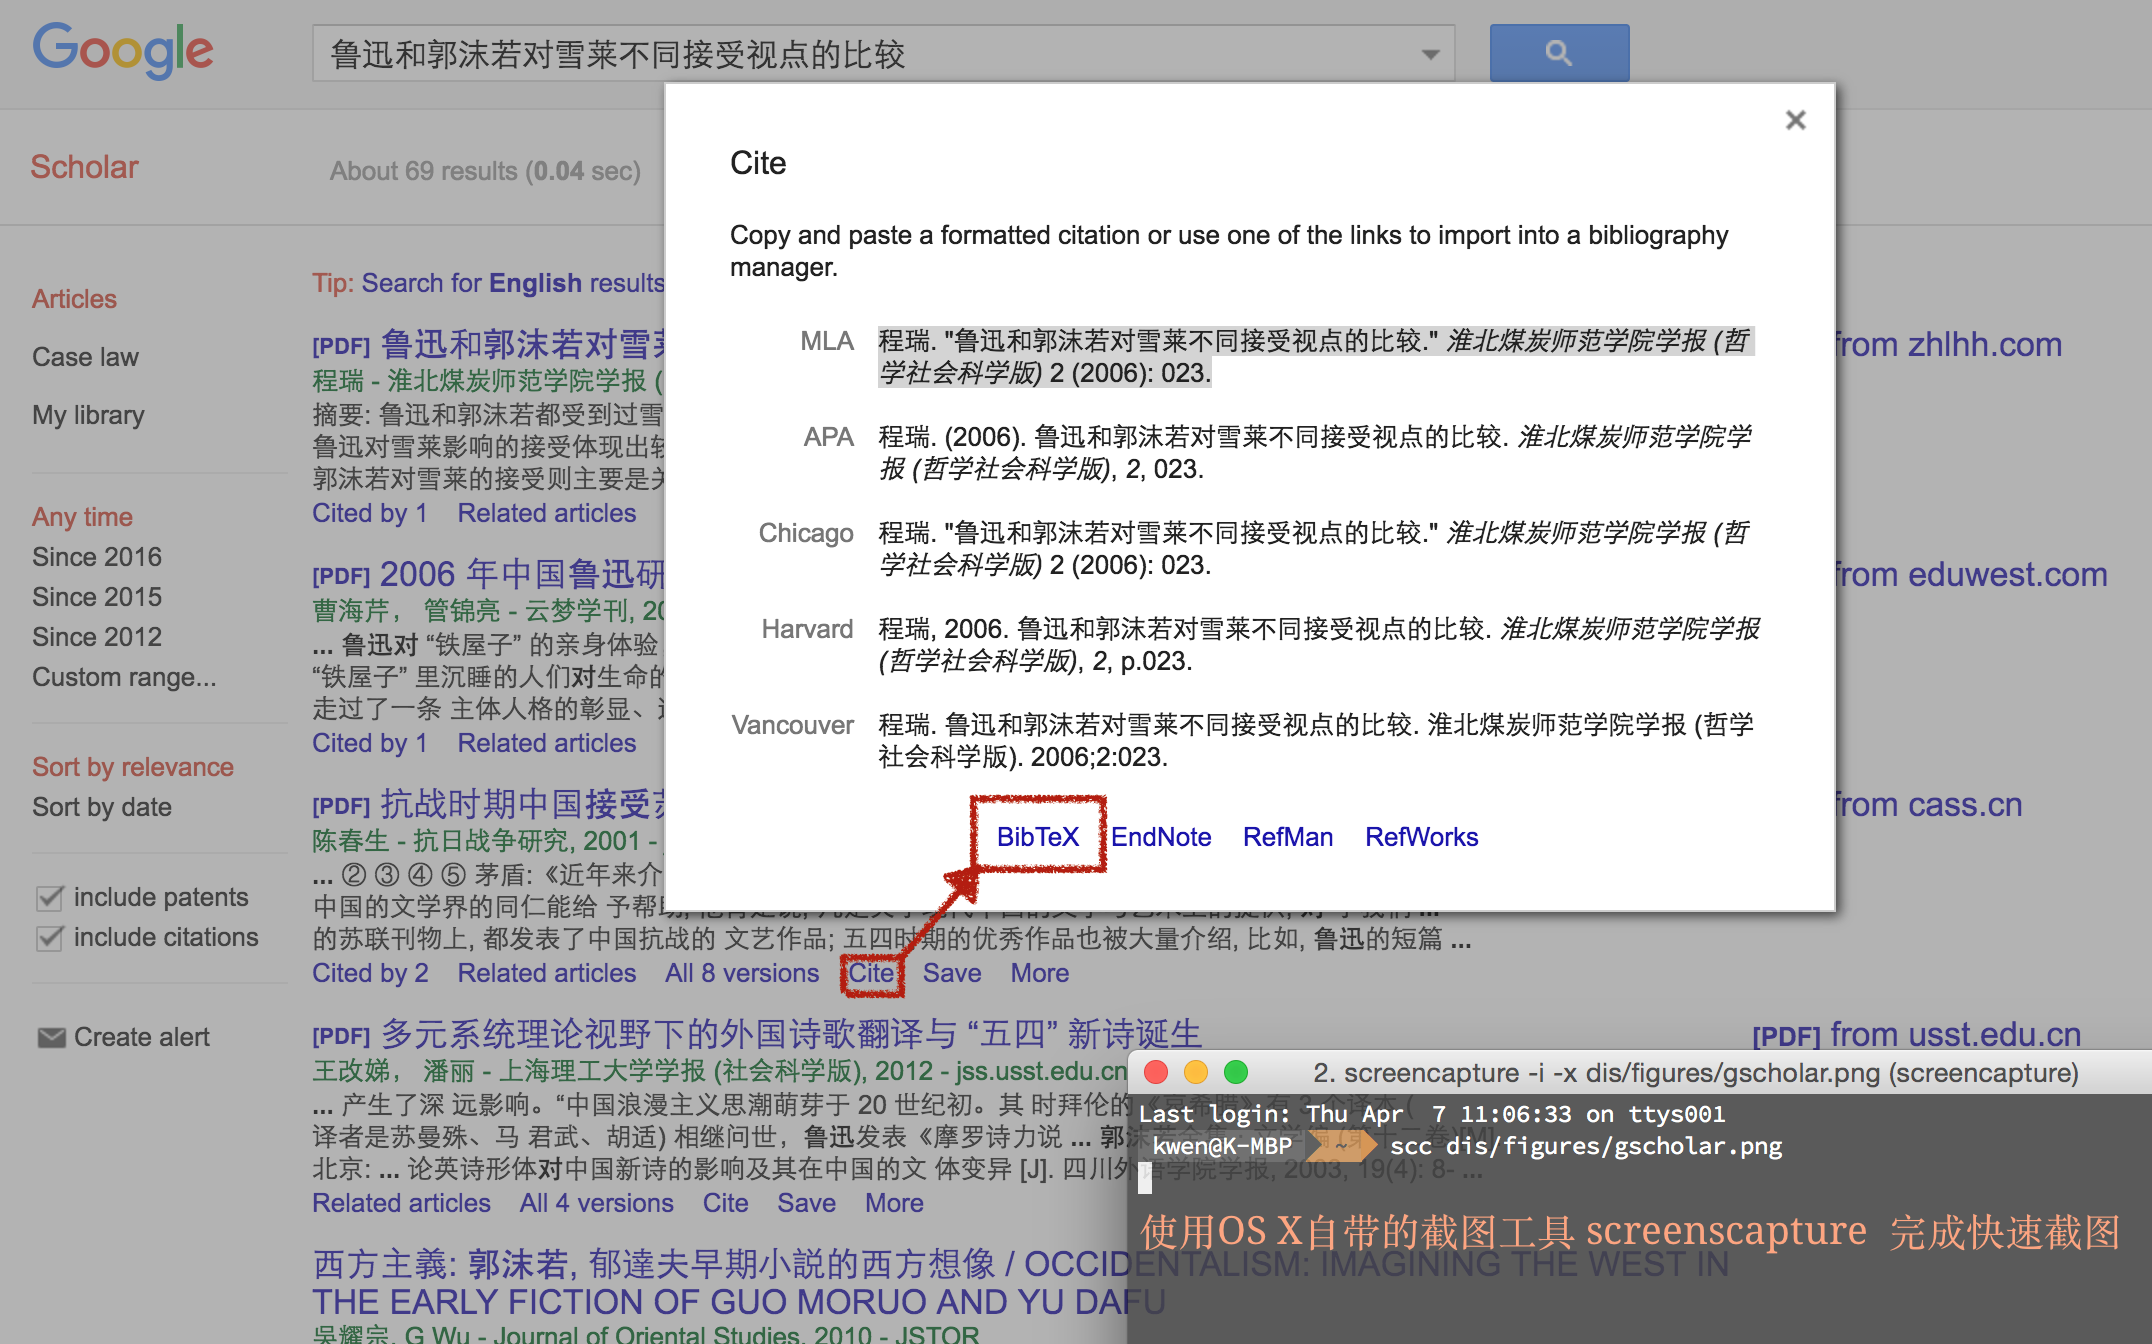
\includegraphics[width=\textwidth]{gscholar.png}
    \caption{使用Google学术查找引文的BibTeX字段}
    \label{fig:gscholar}
\end{figure}

注意,由Google学术提供的文献类型和字段有可能不满足胡海星的设定,
注意调整。
胡海星提供的参考文献样式表中设定的文献类型列出:
\begin{description}
    \item[期刊]          \texttt{@article}
    \item[专著]          \texttt{@book, @inbook}
    \item[译著]          \texttt{@Book, @inBook}
    \item[会议论文集]    \texttt{@proceeding, @inproceeding}
    \item[手册]          \texttt{@manual}
    \item[网页]          \texttt{@webpage, @online}
\end{description}

\begin{itemize}
    \item 比如这是一篇中文期刊\cite{lixiaodong1999}
    \item 这是几篇英文期刊\cite{christine1998, kanamori1998}
    \item 一本中文书\cite{zh-book-1}
    \item 一本中文译著\cite{anwen1988b}
    \item 一本英文书\cite{lamport1994latex, takeuti1973}
    \item 一篇中文inproceeding\cite{nonlinear1996}
    \item 中文proceeding\cite{a2-1}
    \item 英文proceeding\cite{a2-2}
    \item 中文inproceeding\cite{aczel1998}
    \item 一篇学位论文\cite{a4-1} 
    \item 其他资料:手册\cite{ipad}报纸\cite{renminribao}网页\cite{dubash2010}
\end{itemize}

在论文中设置了一个错误或丢失的引用不会引起编译错误,
引擎会在引用标记中设一个问号。
手动编译论文的顺序一般为:
\begin{verbatim}
xelatex main
bibtex main  // 生成参考文献
xelatex main
xelatex main
\end{verbatim}
latexmk 自动化地执行了这些步骤,所以编译时间才需要20余秒之久。

\section{本章小结}

本章划分节比较多,正式行文中请尽量避免。

传播智识,单单借助文字的力量是相对无力的,
即使是日常博文,列表、插图、表格、代码都少不了。
何况是一篇用于申请硕士学位的论文呢?

一篇学位论文集长期的科研工程实践智慧于寥寥数万字。
如何合理规划论文语义和排版元素,
让即便不熟习此领域的后人能在短时间内消化,
继续开物前民,
是同学们应该在论文撰写过程中反复求索的。


